\documentclass[12pt,a4paper,english]{article}
\usepackage{times}
\usepackage[utf8]{inputenc}
\usepackage{babel,textcomp}
\usepackage{mathpazo}
\usepackage{mathtools}
\usepackage{amsmath,amssymb}
\usepackage{ dsfont }
\usepackage{listings}
\usepackage{graphicx}
\usepackage{ mathrsfs }
\usepackage{float}
\usepackage{subfig} 
\usepackage[hyphens]{url}
\usepackage[colorlinks]{hyperref}
\hypersetup{breaklinks=true}
\usepackage[usenames,dvipsnames,svgnames,table]{xcolor}
\usepackage{textcomp}
\definecolor{listinggray}{gray}{0.9}
\definecolor{lbcolor}{rgb}{0.9,0.9,0.9}
\lstset{backgroundcolor=\color{lbcolor},tabsize=4,rulecolor=,language=python,basicstyle=\scriptsize,upquote=true,aboveskip={1.5\baselineskip},columns=fixed,numbers=left,showstringspaces=false,extendedchars=true,breaklines=true,
prebreak=\raisebox{0ex}[0ex][0ex]{\ensuremath{\hookleftarrow}},frame=single,showtabs=false,showspaces=false,showstringspaces=false,identifierstyle=\ttfamily,keywordstyle=\color[rgb]{0,0,1},commentstyle=\color[rgb]{0.133,0.545,0.133},stringstyle=\color[rgb]{0.627,0.126,0.941},literate={å}{{\r a}}1 {Å}{{\r A}}1 {ø}{{\o}}1}

% Use for references
\usepackage[square,comma,numbers]{natbib}
%\DeclareRobustCommand{\citeext}[1]{\citeauthor{#1}~\cite{#1}}

% Fix spacing in tables and figures
%\usepackage[belowskip=0pt,aboveskip=5pt]{caption}
%\setlength{\intextsep}{10pt plus 2pt minus 2pt}

% Change the page layout
%\usepackage[showframe]{geometry}
%\usepackage{layout}
\setlength{\hoffset}{-0.6in}  % Length left
\setlength{\voffset}{-0.7in}  % Length on top
\setlength{\textwidth}{470pt}  % Width /597pt
\setlength{\textheight}{660pt}  % Height /845pt
%\setlength{\footskip}{25pt}

\newcommand{\VEV}[1]{\langle#1\rangle}
\title{FYS-STK4155 - Project 3}
\date{}
\author{ Kristoffer Langstad \footnote{\url{https://github.com/krilangs/FYS-STK4155}}\\ \textit{krilangs@uio.no}}

\begin{document}%\layout
\maketitle
\begin{abstract}
	...
\end{abstract}
\section{Introduction}
\label{sect:Introduction}
Machine learning is a more and more used method for classification problems. One application of machine learning is to create filters that decreases the human dependency for classification. Normally a human is needed to go through data and decide what the classification of an object is. With machine learning the goal is to make this as automated as possible by using suited algorithms and methods. We will look at several methods for classification in this project.

In this project we will study a binary classification problem involving the prediction of pulsar star candidates collected during the HTRU survey from the UCI Machine Learning Repository \cite{UCI}. This data set, called HTRU2, has previously been studied in a scientific paper by \citet{pulsar_art} for finding good filters for classification of pulsars. So some of the results in this paper is used to compare with the results we get. We will use several classification methods from the Scikit-Learn library in Python for classifying the pulsar data, to see which method(s) is the best for classifying these pulsar data. We will explore different approaches from decision trees to random forests, different boosting methods and a couple of other classification methods. For the analysis part we will look at among others the accuracy score, Cohen Kappa score, mean squared error (MSE), confusion matrix and so on.

First we will look at the HRTU2 data set to be evaluated, what it contains and information about the data set. Then in the theory section we will look at the theory of the different classification methods and analysis methods to be used. In the methods section we explain the implementation of the algorithms in Python. Here we first download and read in the data to a Python program. With this program we will look at the data a bit more by looking at the correlation and the information gain
of the data features. Then we split the data into training and test data to be used in the various algorithms. For these algorithms we test to find the best input parameters. In the results section we will present and discuss the classification results, and compare them with the scientific report. Lastly, we give a critical evaluation of the methods on which is the best method on the pulsar data set.

\section{Data}
\label{sect:Data}
The HRTU2 data set we are analyzing is downloaded from the UCI Machine Learning Repository \cite{UCI} as a CSV file. The data file contains feature data about possible pulsar candidates collected during the High Time Resolution Universe (HTRU) survey, and are classified as pulsars (positive, 1) or non-pulsars (negative, 0). 

Pulsar stars are Neutron stars that rotate with such velocity that they emit radio emission that we can detect on Earth. These stars are often very rare, and are interesting to us in the matter of probes of space-time, interstellar-medium and states of matter \cite{UCI}. The beam the pulsars emit when rotating are different from pulsar to pulsar, and they may even vary a little for each rotation. So to find a potential signal candidate, the signals are averaged over many rotations of the pulsars. In most cases the detected signals are caused by noise and radio frequency interference (RFI), and not signals from real pulsars.

The data set contains a total of 17 898 number of instances (161 082 data points), where 1 639 are real pulsar examples and 16 259 are spurious examples caused by noise/RFI. So the real pulsar data examples are a minority positive class. All the data have been checked by human annotators. Each candidate is stored in a separate row and contains 8 continuous variables and the class label (0 or 1):
\begin{enumerate}
	\item Mean of the integrated profile. Renamed: "Mean\_Int".
	\item Standard deviation of the integrated profile. Renamed: "STD\_Int".
	\item Excess kurtosis of the integrated profile. Renamed: "EX\_Kurt\_Int".
	\item Skewness of the integrated profile. Renamed: "Skew\_Int".
	\item Mean of the DM-SNR curve. Renamed: "Mean\_DMSNR".
	\item Standard deviation of the DM-SNR curve. Renamed: "STD\_DMSNR".
	\item Excess kurtosis of the DM-SNR curve. Renamed: "Ex\_Kurt\_DMSNR".
	\item Skewness of the DM-SNR curve. Renamed: "Skew\_DMSNR".
	\item Target\_class. Renamed: "Target".
\end{enumerate}
The first four variables are simple statistics from the integrated pulse profile. They describe the longitude-resolved version of the signal that has been averaged in both time and frequency. The next four are obtained from the DM-SNR curve, and contains the same type of information. Their mathematical definitions can be seen in Table 4 in the scientific paper by \citet{pulsar_art}. In this scientific paper (section 5) there are also more thorough explanations about the pulsar data and how they are produced.

The 8 continuous feature variables are set as the design matrix \textbf{X}, and the class variable are the target vector \textbf{y}. The data set looks to be complete without any NAN values.

\section{Theory}
\label{sect:Theory}
First is a theory part about the classification algorithms we use in the program. Then is a theory part about the evaluation methods we use to evaluate the classification algorithms on the data set.

\subsection{Classification Methods}
\label{subsect:class_methods}
Under follows a brief theory on how each of the classification methods work. In the Python program, the classification algorithms are implemented using their respective function from the Scikit-Learn library with varying input parameters suited for each method.

\subsubsection{Logistic Regression}
\label{subsubsect:LR}
Logistic regression (LR) is used in statistical analysis on a dataset with often several independent variables with a binary outcome. It models the posterior probability of K feature classes by using linear regression to fit data to a logit function yielding a binary output in [0, 1]. When there are more than two outcomes, it is classified by multinomial logistic regression. First is to classify the inputs as class 0 or 1. Here it computes the probability of an observation belonging to the class 1. Then use a logit function for probabilities to classify the elements into the two target classes. Then it defines a boundary threshold for values between 0 and 1, to make sure that all the values are set to 0 or 1. \cite{LR}

\subsubsection{Support Vector Machine}
\label{subsubsect:SVM}
The main idea of support vector machines (SVM) is to find an optimal hyperplane (a line for two feature classes) for K feature classes (making a K-dimensional space) that separates the data points in the target classes. This optimal hyperplane occurs when we have the maximum distance separating the class data points. The support vectors are the data points which are closest to the hyperplane, and has an affect on how the hyperplane looks. The SVM takes the output from the linear function, like the LR method, put now gives it the values [-1, 1]. Then it maximizes the margin between the hyperplane and the data points by using a cost function with a regularization parameter for balancing the loss and the maximization of the margin. Then it minimizes the cost functions with respect to the weights to find the gradients. This is use to update the weights. With no misclassification, the gradients are updated from the regularization parameter. With misclassification, the gradients are updated by adding a loss to the regularization parameter. \cite{SVM}

\subsubsection{Decision Tree}
\label{subsubsect:Tree}
Decision trees (CART) uses the data features to construct a tree-like graph for outcomes and possible events. Here each internal node represents a test on a feature that results in leaf nodes representing the class targets. For decision trees the important part is to choose which features to choose as root node and internal nodes, and how to split the features. To decide the importance of the features, we can use the misclassification error, Gini index or the cross-entropy. The Gini index and cross-entropy are better for numerical optimization since they are differentiable. The Gini index shows how good a split is by how mixed the response classes are in the groups created by the split. The cross-entropy is used to calculate the information gain for a specific feature by the difference between the total outcome entropy and the entropy of a specific feature. The feature with the highest value is chosen as the root node. This is then removed to find the next highest feature for each specific branch. This is repeated until the last internal node. The decision tree use a cost function to find the most homogeneous branch when splitting. The stop point of splitting can also be set by us like choosing a certain maximum depth of the tree from the root to a leaf. Pruning is also used to remove nodes that use features with low importance.

\subsubsection{Bagging}
\label{subsubsect:Bag}
Bagging classification is used to improve CART algorithms by adding bootstrap aggregation and randomization on the classifier. In this project we use bagging on the decision tree classifier. So the bagging classification produces several decision trees to combine several estimates instead of just using the one to try to improve the accuracy score.

\subsubsection{Random Forest}
\label{subsubsect:Forest}
The random forest algorithm produces several decision trees on bootstrapped training samples which differ from each other with low correlation. It takes a fresh sample of $m\approx\sqrt{p}$ predictors/variables at each split in the tree, with $p$ the full set of predictors. From these splits the best is picked to be split further into sub-nodes. This continues until a minimum node size is reached. Then it outputs an ensemble of trees to be used for evaluation.

\subsubsection{Voting Classifier}
\label{subsubsect:Vote}
The voting classifier uses several other classification methods to create an ensemble to try to increase the accuracy score. Since it uses several classification methods it can combine exploit different traits from the used methods. It has two types of voting; hard and soft voting. Hard voting uses the class target with the highest number of votes from the classifiers to be chosen. Soft voting uses the probability vector for each predicted class and are summed up and averaged for each classifier. The class with the highest value is then chosen. \cite{vote}

\subsubsection{AdaBoost}
\label{subsubsect:Ada}
The AdaBoost uses adaptive boosting to sequentially apply weak classifiers to repeatedly modified data sets by combining them into a single better classifier through a weighted majority vote. In this project we use the AdaBoost on the decision tree classifier. The algorithm puts more weight on instances that are hard to classify and less on the instances that are handled well. The algorithm first initializes the observation weights. Then the classifier is fit to the training data using the weights. Then it computes the weighted error rate and another weight given to the classifier to produce the final output classifier. This new classifier is then weighted on the previous classifier, such that the new tree hopefully has a better prediction. The new model is then the two trees added together. This procedure is repeated several times of a given number of iterations.  \cite{hastie2009}

\subsubsection{Gradient Boosting}
\label{subsubsect:Grad}
The Gradient boosting is another method for converting weak classifiers into stronger classifiers. The Gradient boost is similar to the AdaBoost, where the biggest difference is how the Gradient identifies the shortcomings of the weak classifiers. The AdaBoost uses high weight data points, while Gradient boosting do the same with gradients in the loss function. This method allows for a more open and specified cost function for optimization that fits the classification problem we are dealing with. \cite{hastie2009} 

\subsubsection{Extreme Gradient Boosting}
\label{subsubsect:XGB}
The Extreme Gradient Boosting (XGBoost) is an optimized distributed gradient boosting library made to be highly efficient, flexible and portable. It provides a fast and accurate parallel tree boosting \cite{lect_trees}. The XGBoost takes into consideration the potential loss for the possible splits to make a new branch by looking at distributions of the features for all data points in a leaf. This is used to decrease the space of possible feature splits search. This method involves many hyperparameters for optimal tuning. 

\subsection{Evaluation Methods}
\label{subsect:eval_methods}
Since we have a binary classification problem (dichotomous target variable), we can compute the point-biserial correlation coefficient $r_{pb}$ between the data features (sect. 5.1.3 in \citet{pulsar_art}). This is a measurement of the linear correlation between the continuous features and the binary target, which yields values between -1 and 1. This is calculated as 
\begin{equation}
\label{eq:point_biserial}
r_{pb}=\frac{\overline{x}_1-\overline{x}_2}{\sigma}\cdot\sqrt{\frac{n_2\cdot n_1}{n(n-1)}},
\end{equation}
where $n$ is the total number of samples, $\overline{x}_i$ is the mean value of a feature group $i$ and $\sigma$ is the sample standard deviation. This is calculated with the \textit{pointbiserialr} function from the Scipy.stats library in Python on the design matrix \textbf{X} and target \textbf{y}. This is calculated for each of the 8 features.

For more information on the correlation in the data set, we can look at the entropy and information gain. The entropy is calculated as (\cite{pulsar_art})
\begin{equation*}
H(x_i)=-\sum_{j\in x_i}P(j)\log_2P(j),
\end{equation*}
where $j$ corresponds to each value that a feature group $x_i$ can take and $P(j)$ is the probability of $j$ occurring. The conditional entropy of the feature $x_i$ given target \textbf{y} is 
\begin{equation*}
H(x_i|\textbf{y})=-\sum_{y\in\textbf{y}}P(y)\sum_{j\in x_i}P(j|y)\log_2P(j|y).
\end{equation*} 
With these definitions we define the information gain (mutual information) for a given feature as the difference between the total outcome entropy and the entropy of the given feature as
\begin{equation}
\label{eq:inf_gain}
I(x_i:\textbf{y})=H(x_i)-H(x_i|\textbf{y}).
\end{equation}
The information gain is a measure of the correlation between a feature and the target which detects non-linearities or the amount of information that one feature provides about another. This is calculated using the \textit{mutual\_info\_classif} function from the Scikit-Learn library.

For classification we measure the performance of the model with the accuracy score which is the number of correct predictions divided by the total number of predictions:
\begin{equation}
\label{eq:accuracy}
\text{Accuracy}=\frac{\sum_{i=1}^{n}I(t_i=y_i)}{n}
\end{equation}
Here $n$ is the total number of predictions, $t_i$ is the predicted target, $y_i$ is the class target and $I$ is an indicator function as
\[I=\begin{cases}
1, \text{ if } t_i=y_i\\
0, \text{ if } t_i\neq y_i
\end{cases}.\]
The optimal accuracy score is 1, which means that the prediction fits the data perfect. With the \textit{cross\_val\_score} function in the Scikit-Learn library we also calculate the test cross-validation score with 5 folds with the test data for the chosen classifier.

Another score function is the Cohen Kappa score, which takes into account the accuracy that would have happened through random predictions. It measures how well the classifier actually performs, and the best score is 1 as for the accuracy score. The Kappa score is calculated as (\cite{kappa})
\begin{equation}
\label{eq:kappa}
\kappa=\frac{\text{Observed Accuracy} - \text{Expected Accuracy}}{1-\text{Expected Accuracy}}=\frac{p_a-p_e}{1-p_e}.
\end{equation}

For evaluating the error in the predicted values we also calculate the mean squared error (MSE) as
\begin{equation}
\label{eq:mse}
MSE(\textbf{y},\tilde{\textbf{y}})=\frac{1}{n}\sum_{i=1}^{n}(y_i-\tilde{y}_i)^2,
\end{equation}
where $\tilde{y}_i$ is the predicted value and $y_i$ is the true value of the variables being predicted of the $i$-th sample.

For more error evaluation we also look at the variance of the predicted values, which is a measure on how far the predictions are spread out from their average value. It is also the represented as the square of the standard deviation. The variance is calculated as
\begin{equation}
\label{eq:var}
Var(\tilde{\textbf{y}})=\frac{1}{n}\sum_{i=1}^{n}(\tilde{y}_i-\frac{1}{n}\sum_{i=1}^{n}\tilde{y}_i)^2.
\end{equation}

Then we have the bias error, which is the difference between the expected value and the true value. The bias squared is calculated as
\begin{equation}
\label{eq:bias}
Bias(\textbf{y},\tilde{\textbf{y}})=\frac{1}{n}\sum_{i=1}^{n}(y_i-\frac{1}{n}\sum_{i=1}^{n}\tilde{y}_i)^2.
\end{equation}

With the \textit{classification\_report} function from the Scikit-Learn library we can compute a classification report. This classification report contains various averages for the two target classes 0 and 1 (Table 10 in \citet{pulsar_art}):
\begin{enumerate}
	\item Precision: Fraction of retrieved instances that are positive: \[\frac{TP}{TP+FP}\]
	\item Recall: Fraction of positive instances that are retrieved:
	\[\frac{TP}{TP+FN}\]
	\item F1-score: Measure of accuracy that considers both precision and recall:
	\[2\times\frac{\text{Precision}\times\text{Recall}}{\text{Precision}+\text{Recall}}\]
	\item Support: Predictive positive rate=fraction of positively predicted examples:
	\[\frac{TP+FP}{N}\]
	\item Accuracy: The accuracy score of the F1-score only (in our case).
	\item Macro avg: Average of the unweighted mean per label.
	\item Weighted avg: Average of the support-weighted mean per label.
\end{enumerate}
Here we use the prediction results to calculate the precision and recall. They are given as:
\begin{enumerate}
\label{enu:outcomes}
	\item[] Positive (P) - Observation is positive.
	\item[] Negative (N) - Observation is negative.
	\item[] True Positive (TP) - Observation is positive, and prediction is positive.
	\item[] True Negative (TN) - Observation is negative, and prediction is negative.
	\item[] False Positive (FP) - Observation is negative, and prediction is positive.
	\item[] False Negative (FN) - Observation is positive, and prediction is negative.
\end{enumerate}

These outcomes are also used in the confusion matrix for binary outcomes. The confusion matrix will look like Figure \ref{fig:conf_mat}. The values in the confusion matrix are normalized such that the total value of the rows equals 1. The optimal values are TN=1, FP=0, FN=0 and TP=1. This means that all the predictions are correct.

\begin{figure}[h!]
	\centering\includegraphics[width=0.4\linewidth]{Conf_mat.png}
	\caption{Confusion matrix describing the outcomes of the pulsars. Explanation of the outcomes in \ref{enu:outcomes}. \label{fig:conf_mat}}
\end{figure} 

Another plot we can compute with these prediction results, is the Receiver Operating Characteristic (ROC) curve. This plots the true positive rate (sensitivity) as a function of the false positive rate (specificity) for the class 0, class 1, micro-average and macro-average for the classifier. The earlier the true positive rate reaches 1.0, the better the accuracy of the classifier.

By plotting the cumulative gain of the class targets as functions of the percentage of samples, we can see how effective the classifier is at predicting the class targets as the percentage of the samples vary.

For the XGBoost we can look at the feature importance when building the trees. This counts the number of times a feature is split across all boosting trees. With the \textit{plot\_importance} function in the XGBoost library, we get a bar graph over how many times each feature appear in the trees.


\section{Methods}
\label{sect:Methods}
The programming is done in Python 3.7 in the program \textit{classif.py} found at the GitHub repository (\ref{sect:Appendix}), among with the pulsar data file and produced figures.

\subsection{Analyzing the Data}
\label{subsect:analysis}
We start by reading in the downloaded CSV file \textit{pulsar\_stars.csv} of the pulsar candidates in the program. Then we rename the feature variables to be shorter (as seen in the Data section \ref{sect:Data}). By using the panda-library, we do an analysis of the data set to make sure that the data file is complete and read in correct. We also check the correlation between the data features by plotting a correlation heatmap using the seaborn-library. Next, we create the design matrix \textbf{X} and target vector \textbf{y} as mentioned in the Data section (\ref{sect:Data}). As in the scientific report \cite{pulsar_art}, we calculate the point-biserial correlation coefficient of the data features with the design matrix and target vector. The design matrix and target vector are then split into training and test data with 27\% test data. Then we scale the design training and test data with respect to the training data. With the training data we calculate the information gain of the features.

\subsection{Classification}
\label{subsect:classif}
Then we implement all the classification methods we explained in the Theory section (\ref{subsect:class_methods}) into our program using the Scikit-Learn and xgboost libraries. All classifiers have random\_state=42, for reproduction of results. The used classifiers include (input parameters that are not covered, uses the default parameters):
\begin{enumerate}
	\item Logistic Regression (LR): Where we use the \textit{liblinear}-solver.
	\item Support Vector Machine (SVM): Where we use probability=True to calculate probability estimates. Set gamma="auto", which is a kernel coefficient as 1/n\_features.
	\item Decision Tree: Where we set the maximum depth of the tree to 6, since this give the best results. Here we also plot a decision tree for visualization only.
	\item Bagging: Where we use bagging on the decision tree with bootstrap, 500 estimators in the ensemble, maximum 200 samples to train on each base estimator and use all processors to run the jobs in parallel (for speed).
	\item Random Forest: With 500 estimators.
	\item Voting classifier: Use both hard and soft voting separately on all of the mentioned classifier methods mentioned above together (1-5), and use all processors to run the jobs in parallel.
	\item AdaBoost: Use AdaBoost on the decision tree with 200 estimators and the "SAMME.R" real boosting algorithm \citep{SAMMER}.
	\item Gradient boosting: Where we use the exponential loss function to be optimized, 200 estimators and a maximum depth of 9 for the number of nodes in the tree.
	\item XGBoost: Where we use the "multi:softprob" learning objective with 2 classes (since binary problem), which does a multiclass classification and outputs a vector containing predicted probabilities of each data point to each class. We also use 250 estimators and set maximum depth of the tree to 5. Here we also plot the visualization of the first decision tree in this algorithm, and plot the feature importance of the trees.
	\item Voting classifier: Where we use the soft voting classifier on the classification methods yielding the highest accuracy score. This include decision tree, random forest, AdaBoost, Gradient boost and XGBoost.
\end{enumerate}

For each of the classification methods above, we do the same evaluations of the pulsar data set. The various evaluations are explained in the theory section (\ref{subsect:eval_methods}). We fit the classification methods to the training data. Then we use the test data to make a prediction of the class labels. With this prediction we calculate the MSE, variance, bias, accuracy score and the Cohen Kappa score. We also make a classification report containing various averages for the classification methods. Then we plot the confusion matrix of the predicted results of the pulsars. With the test data we calculate the cross-validation score with 5 folds. Then we plot the ROC curve for the classification methods for the sensitivity as function of the specificity. For the hard voting classification we use the prediction, while for the others we use the probability estimation of the test data to make the ROC curve plot. Lastly we use the probability estimate to plot the cumulative gain for the class targets as functions of the percentage of the samples.

\section{Results}
\label{sect:Results}
For comparison of our results, we compare with the results in the scientific report by \citet{pulsar_art}.

\subsection{Results of the Data Analysis}
\label{subsect:Res_analysis}
In Figure \ref{fig:heatmap} we see a heatmap of the correlations between the features (from -1 to 1) in the pulsar data set. A score of 1 means the features are perfectly correlated, while a score of -1 means a perfect anti-correlation between the features. If the score is 0 then the features are independent on each other. From this map we see a high positive correlation between:
\begin{itemize}
	\item Excess kurtosis of the integrated profile \& Skewness of the integrated profile (0.95).
	\item Excess kurtosis of the DM-SNR curve \& Skewness of the DM-SNR curve (0.92).
	\item Mean of the DM-SNR curve \& Standard deviation of the DM-SNR curve (0.80).
\end{itemize}
This means that these features are highly correlated to each other. The diagonal is the correlation of the feature with it self, which is obviously 1. We also see a high negative correlation between:
\begin{itemize}
	\item Mean of the integrated profile \& Excess kurtosis of the integrated profile (-0.87).
	\item Standard deviation of the DM-SNR curve \& Excess kurtosis of the DM-SNR curve (-0.81).
	\item Mean of the integrated profile \& Skewness of the integrated profile (-0.74).
\end{itemize}

\begin{figure}[htbp!]
	\centering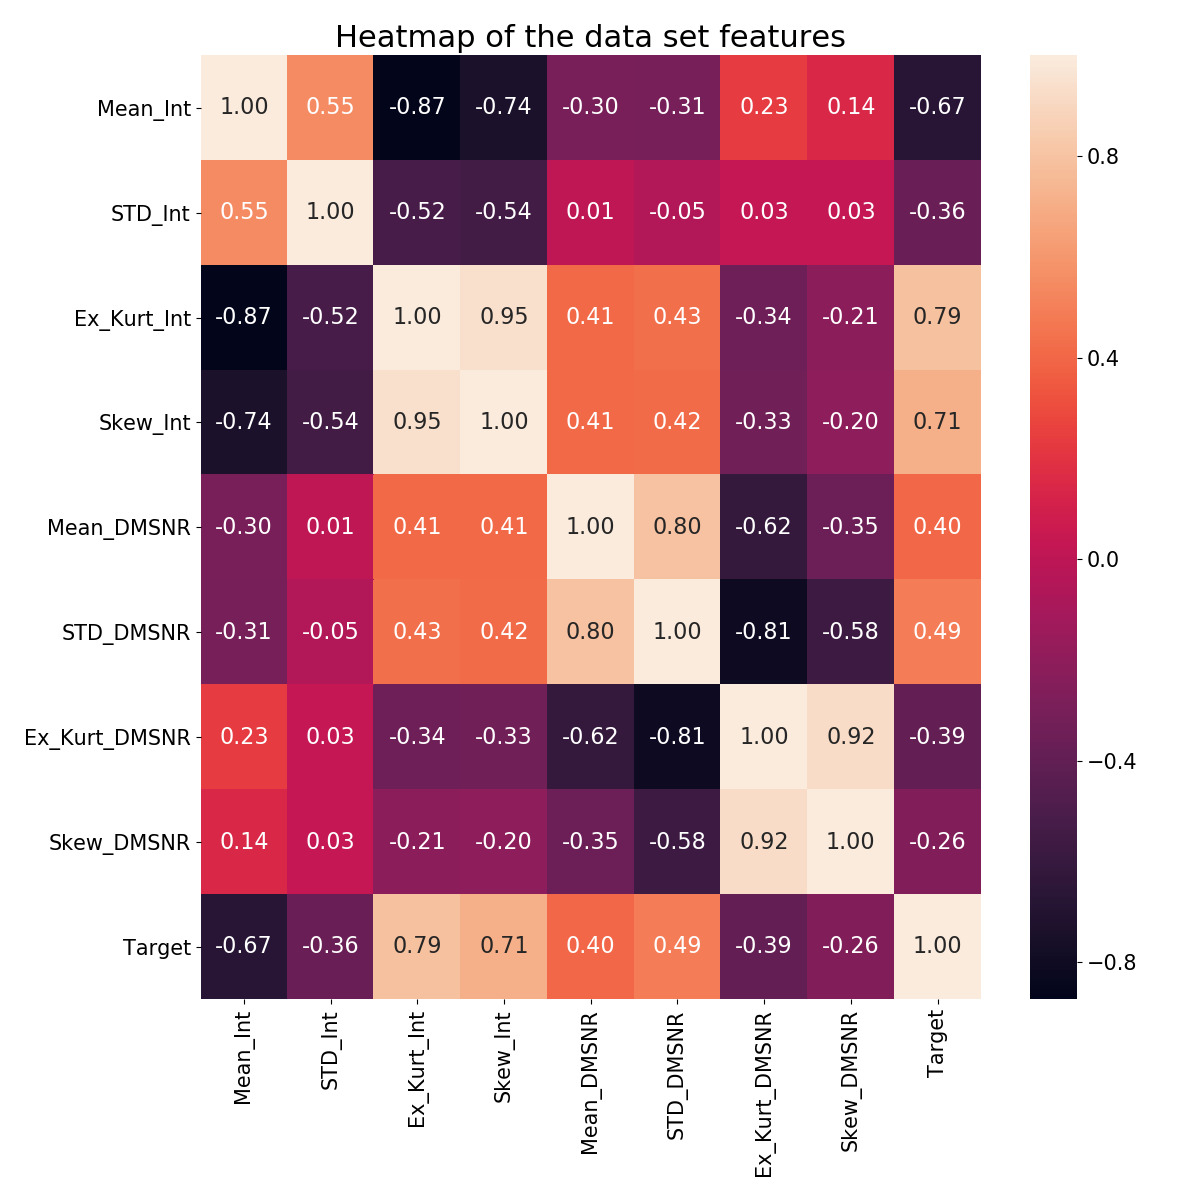
\includegraphics[width=0.8\linewidth]{heatmap.png}
	\caption{Here we see a heatmap of the correlations between the features in the pulsar data set.\label{fig:heatmap}}
\end{figure} 

The point-biserial correlation coefficient in equation \ref{eq:point_biserial}, which measures the linear correlation between the features and the class target, for the features can be seen in Table \ref{tab:correlations}. Here we see that especially the mean, excess kurtosis and skewness of the integrated profile give strong correlations ($>|0.5|$) to the class targets. This is the same values as in Table 6 in the scientific article by \citet{pulsar_art} when rounding to the same number of digits, except for the skewness of the DM-SNR curve where we get $\approx-0.259$ while they got $\approx-0.230$. We also see that none of the features are independent on the target class.

After splitting the data set into training and test data and scaling the training data, we calculated the information gain of the features as explained in the Data section \ref{sect:Data}. The information gains of the features can be also be seen in Table \ref{tab:correlations} (the rightmost values). There we see that the features of the integrated profile (except the STD) gives the higher values, which means that these features seems to be the most important. The difference between the integrated profile features and the DM-SNR curve features are not that different, so all the feature have to be considered.

\begin{table}[htbp!]
	\centering
	%\hspace{-1cm}
	\begin{tabular}{ |c|c|c| }
		\hline \rule{0pt}{13pt}
		Feature & $r$-correlation & Information gain \\
		\hline \rule{0pt}{13pt}
		Mean of the integrated profile & -0.673181 & 0.191635 \\
		\hline \rule{0pt}{13pt}
		Standard deviation of the integrated profile & -0.363708 & 0.088278 \\
		\hline \rule{0pt}{13pt}
		Excess kurtosis of the integrated profile & 0.791591 & 0.226438 \\
		\hline \rule{0pt}{13pt}
		Skewness of the integrated profile & 0.709528 & 0.194512 \\
		\hline \rule{0pt}{13pt}
		Mean of the DM-SNR curve & 0.4008761 & 0.114824 \\
		\hline \rule{0pt}{13pt}
		Standard deviation of the DM-SNR curve & 0.491535 & 0.119248 \\
		\hline \rule{0pt}{13pt}
		Excess kurtosis of the DM-SNR curve & -0.390816 & 0.113393 \\
		\hline \rule{0pt}{13pt}
		Skewness of the DM-SNR curve & -0.259117 &0.115064 \\
		\hline
	\end{tabular}	
	\caption{Table for the point-biserial correlation coefficient in equation \ref{eq:point_biserial} for each feature on the pulsar data set. This is a measurement of the linear correlation between the features and the class target. Specially three features give strong correlations ($>|0.5|$) to the class targets; the mean, excess kurtosis and skewness of the integrated profile. To the right we see the information gain of the features. The information gain is a measure of the correlation between a feature and the target which detects non-linearities. Here we see that the features of the integrated profile (mostly) gives the higher information gain, which means these are the most important features. \label{tab:correlations}}
\end{table}

\subsection{Results of the Classification Analysis}
\label{subsect:Res_class}
...
\begin{table}[htbp!]
	%\centering
	\hspace{-1.5cm}
	\begin{tabular}{ |c|c|c|c|c|c|c|c| }
		\hline \rule{0pt}{13pt}
		Model & Accuracy & $\kappa$-score & Max CV score & Mean CV score & MSE & Variance & Bias \\
		\hline \rule{0pt}{13pt}
		LR & 0.977654 & 0.856473 & 0.984504 & 0.977030 & 0.022346 & \textbf{0.072618} & 0.083076 \\
		\hline \rule{0pt}{13pt}
		SVM & 0.978481 & 0.862088 & \textbf{0.986570} & 0.978892 & 0.021519 & 0.072967 & 0.083066 \\
		\hline \rule{0pt}{13pt}
		Decision Tree & 0.979723 & 0.874138 & 0.981386 & 0.977859 & 0.020277 & 0.078152 & \textbf{0.082955} \\
		\hline \rule{0pt}{13pt}
		Bagging & 0.977033 & 0.853283 & 0.985537 & 0.977857 & 0.022967 & 0.073489 & 0.083051 \\
		\hline \rule{0pt}{13pt}
		Random Forest & 0.979930 & 0.873158 & 0.983471 & 0.978272 & 0.020070 & 0.075223 & 0.083008 \\
		\hline \rule{0pt}{13pt}
		Voting (Hard) & 0.978481 & 0.862979 & 0.985537 & 0.979305 & 0.021519 & 0.074010 & 0.083037 \\
		\hline \rule{0pt}{13pt}
		Voting (Soft) & 0.979516 & 0.869426 & 0.985537 & 0.979513 & 0.020484 & 0.073836 & 0.083042 \\
		\hline \rule{0pt}{13pt}
		AdaBoost & 0.980550 & 0.878510 & 0.98240 & 0.979308 & 0.019450 & 0.077121 & 0.082971 \\
		\hline \rule{0pt}{13pt}
		Gradient Boost & \textbf{0.981378} & \textbf{0.883433} & 0.985537 & 0.979720 & \textbf{0.018622} & 0.076777 & 0.082977 \\
		\hline \rule{0pt}{13pt}
		XGBoost & 0.980757 & 0.878907 & 0.983471 & 0.979721 & 0.019243 & 0.075914 & 0.082994 \\
		\hline \rule{0pt}{13pt}
		Voting (Best) & 0.980964 & 0.879825 & 0.984504 & \textbf{0.980134} & 0.019036 & 0.075396 & 0.083004 \\
		\hline
	\end{tabular}	
	\caption{Table for the evaluation values for all the used classifiers on the pulsar data set. From left to right: The accuracy score, the Cohen Kappa score, highest cross-validation score for 5 folds, the mean cross-validation score, MSE, variance and bias. The values in bold font are the best values for that evaluation value. Here we see Gradient boost has the best accuracy, Cohen Kappa score and MSE. The other eval values are not as important as these, and the differences for the other best compared to gradient boost are not that different. From this analysis we can conclude that the gradient boost is the best classifier for our pulsar data set case. \label{tab:classifiers}}
\end{table}


\section{Conclusion}
\label{sect:Conclusion}
...
\appendix
\section{Appendix}
\label{sect:Appendix}
Link to GitHub repository:\\
\url{https://github.com/krilangs/FYS-STK4155/tree/master/Project3}

\bibliographystyle{plainnat}
\bibliography{myrefs}
\end{document}
